\documentclass{article}
\usepackage{tikz}
\usepackage{pgf}
\usepackage{graphicx}
\usepackage{xcolor}
\usetikzlibrary{calc}
\usetikzlibrary{external}

\colorlet{ecol}{white!80!yellow}
\colorlet{acol}{white!80!blue}
\colorlet{agcol}{white!50!orange}
%\newcommand{\entity}[1]{ellipse (1 and 0.6) node[align=center] {#1}}
\newcommand{\entity}[1]{++(-1,-0.55) rectangle ++(2,1.1) node[midway, align=center] {#1}}
\newcommand{\activity}[1]{++(-1,-0.55) rectangle ++(2,1.1) node[midway, align=center] {#1}}
\newcommand{\agent}[1]{++(-1,-0.55) -- ++(2,0) -- ++(0,0.7) -- ++(-1,0.4) -- ++(-1,-0.4) -- ++(0,-0.7) node[midway, align=center, xshift=1cm, yshift=0.1cm] {#1}}

\tikzexternalize

\begin{document}
This file collects images using TikZ/pgf.
The image(s) will be set when using
\texttt{pdflatex -shell-escape figure.tex}

Please remove the image-pdf beforehand, otherwise it may not be updated properly.


\tikzsetnextfilename{workflow-backwards}
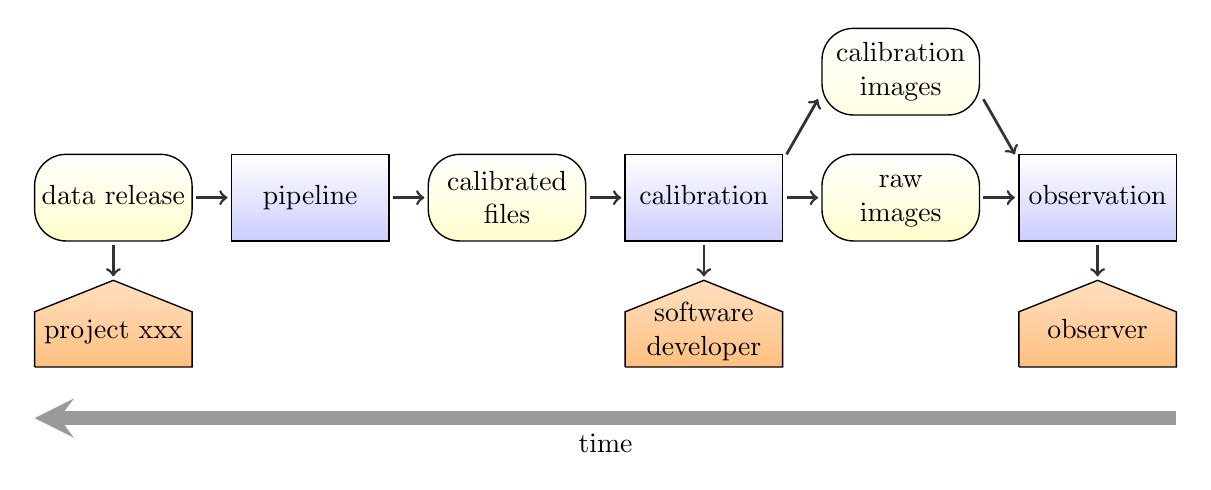
\begin{tikzpicture}
\tikzstyle{astyle}=[line width=0.5pt, rounded corners=0pt, bottom color=acol, top color=white]
\tikzstyle{estyle}=[line width=0.5pt, rounded corners=0.4cm, bottom color=ecol, top color=white]
\tikzstyle{agstyle}=[line width=0.5pt, rounded corners=0pt, bottom color=agcol, top color=white]
\tikzstyle{basic}=[line width=1pt]
\tikzstyle{arrow}=[line width=1pt, black!80, ->]

\coordinate (A) at (0,0);
\coordinate (B) at ($(A)+(2.5,0)$);
\coordinate (C) at ($(B)+(2.5,0)$);
\coordinate (D) at ($(C)+(2.5,0)$);
\coordinate (E) at ($(D)+(2.5,0)$);
\coordinate (F) at ($(E)+(2.5,0)$);

\draw[estyle] (A) \entity{\vphantom{gh}data release};
\draw[arrow] (A) ++(1.05,0) -- ++(0.4,0);
\draw[astyle] (B) \activity{\vphantom{gh}pipeline};
\draw[arrow] (B) ++(1.05,0) -- ++(0.4,0);
\draw[estyle] (C) \entity{\vphantom{gh}calibrated\\files};
\draw[arrow] (C) ++(1.05,0) -- ++(0.4,0);
\draw[astyle] (D) \activity{\vphantom{gh}calibration};

\draw[arrow] (D) ++(1.05,0) -- ++(0.4,0);
\draw[estyle] (E) \entity{\vphantom{gh}raw\\images};

\draw[arrow] (E) ++(1.05,0) -- ++(0.4,0);
\draw[astyle] (F) \activity{\vphantom{gh}observation};

% add calibration images as well
\draw[arrow] (D) ++(1.05,0.55) -- ++(0.4,0.7);
\draw[estyle] (E) ++(0,1.6) \entity{\vphantom{gh}calibration\\images};
\draw[arrow] (E) ++(1.05,1.25) -- ++(0.4,-0.7);


% add agents
\draw[arrow] (A) ++(0,-0.6) -- ++(0,-0.4,0);
\draw[agstyle] (A)++(0,-1.6) \agent{\vphantom{gh}project xxx};

\draw[arrow] (D) ++(0,-0.6) -- ++(0,-0.4,0);
\draw[agstyle] (D)++(0,-1.6) \agent{\vphantom{gh}software\\developer};

\draw[arrow] (F) ++(0,-0.6) -- ++(0,-0.4,0);
\draw[agstyle] (F)++(0,-1.6) \agent{\vphantom{gh}observer};

% time arrow
\draw[line width=5pt, black!40, stealth-] (-1,-2.8) -- ++(14.5,0) node[below, black, pos=0.5] {time};
\end{tikzpicture}

\end{document}
